\section{Introduction}\label{sec:intro}
The modern day power grid is an important societal infrastructure; failure to which can result in significant impact on national and economic security of a nation~\cite{NAP,ref1,raissa_2012}. The inclusion of ICT in the SCADA network has increased the resiliency and facilitated self healing capabilities of the power grid~\cite{alex2012}. This has been made possible through the large connected communication network with several remote access points enabling coordinated monitoring and control functions on the power grid~\cite{smart2005}. However, this has exposed the system to numerous possibilities of cyber threat increasing the risk of a combined catastrophic failure of the power grid along with the communication network~\cite{cigre2007}. Therefore, the smart power grid consisting of the traditional power system with the intertwined ICT elements is identified as a critical interdependent infrastructure where a failure in either network can result in severe impact on the combined system~\cite{stanley_2018}. 

The usage of standardized communication protocol in the SCADA system has opened up several vulnerabilities in the commonly used protocols like distributed network protocol (DNP) and IEC 61850~\cite{iec61850}. These may be known and zero-day type which can be exploited by an adversary to gain unauthorized access to control assets in the SCADA system~\cite{wang1}. For example in the cyber physical system depicted in Fig.~\ref{fig:cyber-physical} the lower part represents the physical power system. The upper part denotes the hierarchical cyber system or the SCADA network associated with the power grid. The substations communicate with the regional control centers through Ethernet communication protocol, the control centers interchange information using the inter control center protocol (ICCP) and also communicate with the transmission operator (TO) through Ethernet routers. In such a setup, an intruder can exploit the vulnerabilities of the control center or substation LAN to gain administrator privilege in one of the human machine interfaces (HMIs)~\cite{ten_main}. By obtaining access, the control commands might be manipulated to operate the circuit breakers in the physical power system resulting in instability in the grid from load-generation imbalance~\cite{attack}. Often such attack can cause cascading events in the system leading to widespread blackout as in the case of Stuxnet malware attack in Ukraine in 2015~\cite{ukraine1,ukraine2}. This is due to the fact that the power system is operated with security analysis performed for at most $2$ contingencies. A planned cyber attack can lead to multiple contingencies at the same time exacerbating the disturbance in the grid. In addition to that an adversary can gain access to the intelligent electronic devices (IEDs) connected to the substation LAN and create a man-in-the-middle attack by injecting false data or modifying information coming from the IEDs to the substation servers~\cite{maninmiddle}.
\begin{figure}
	\centering
	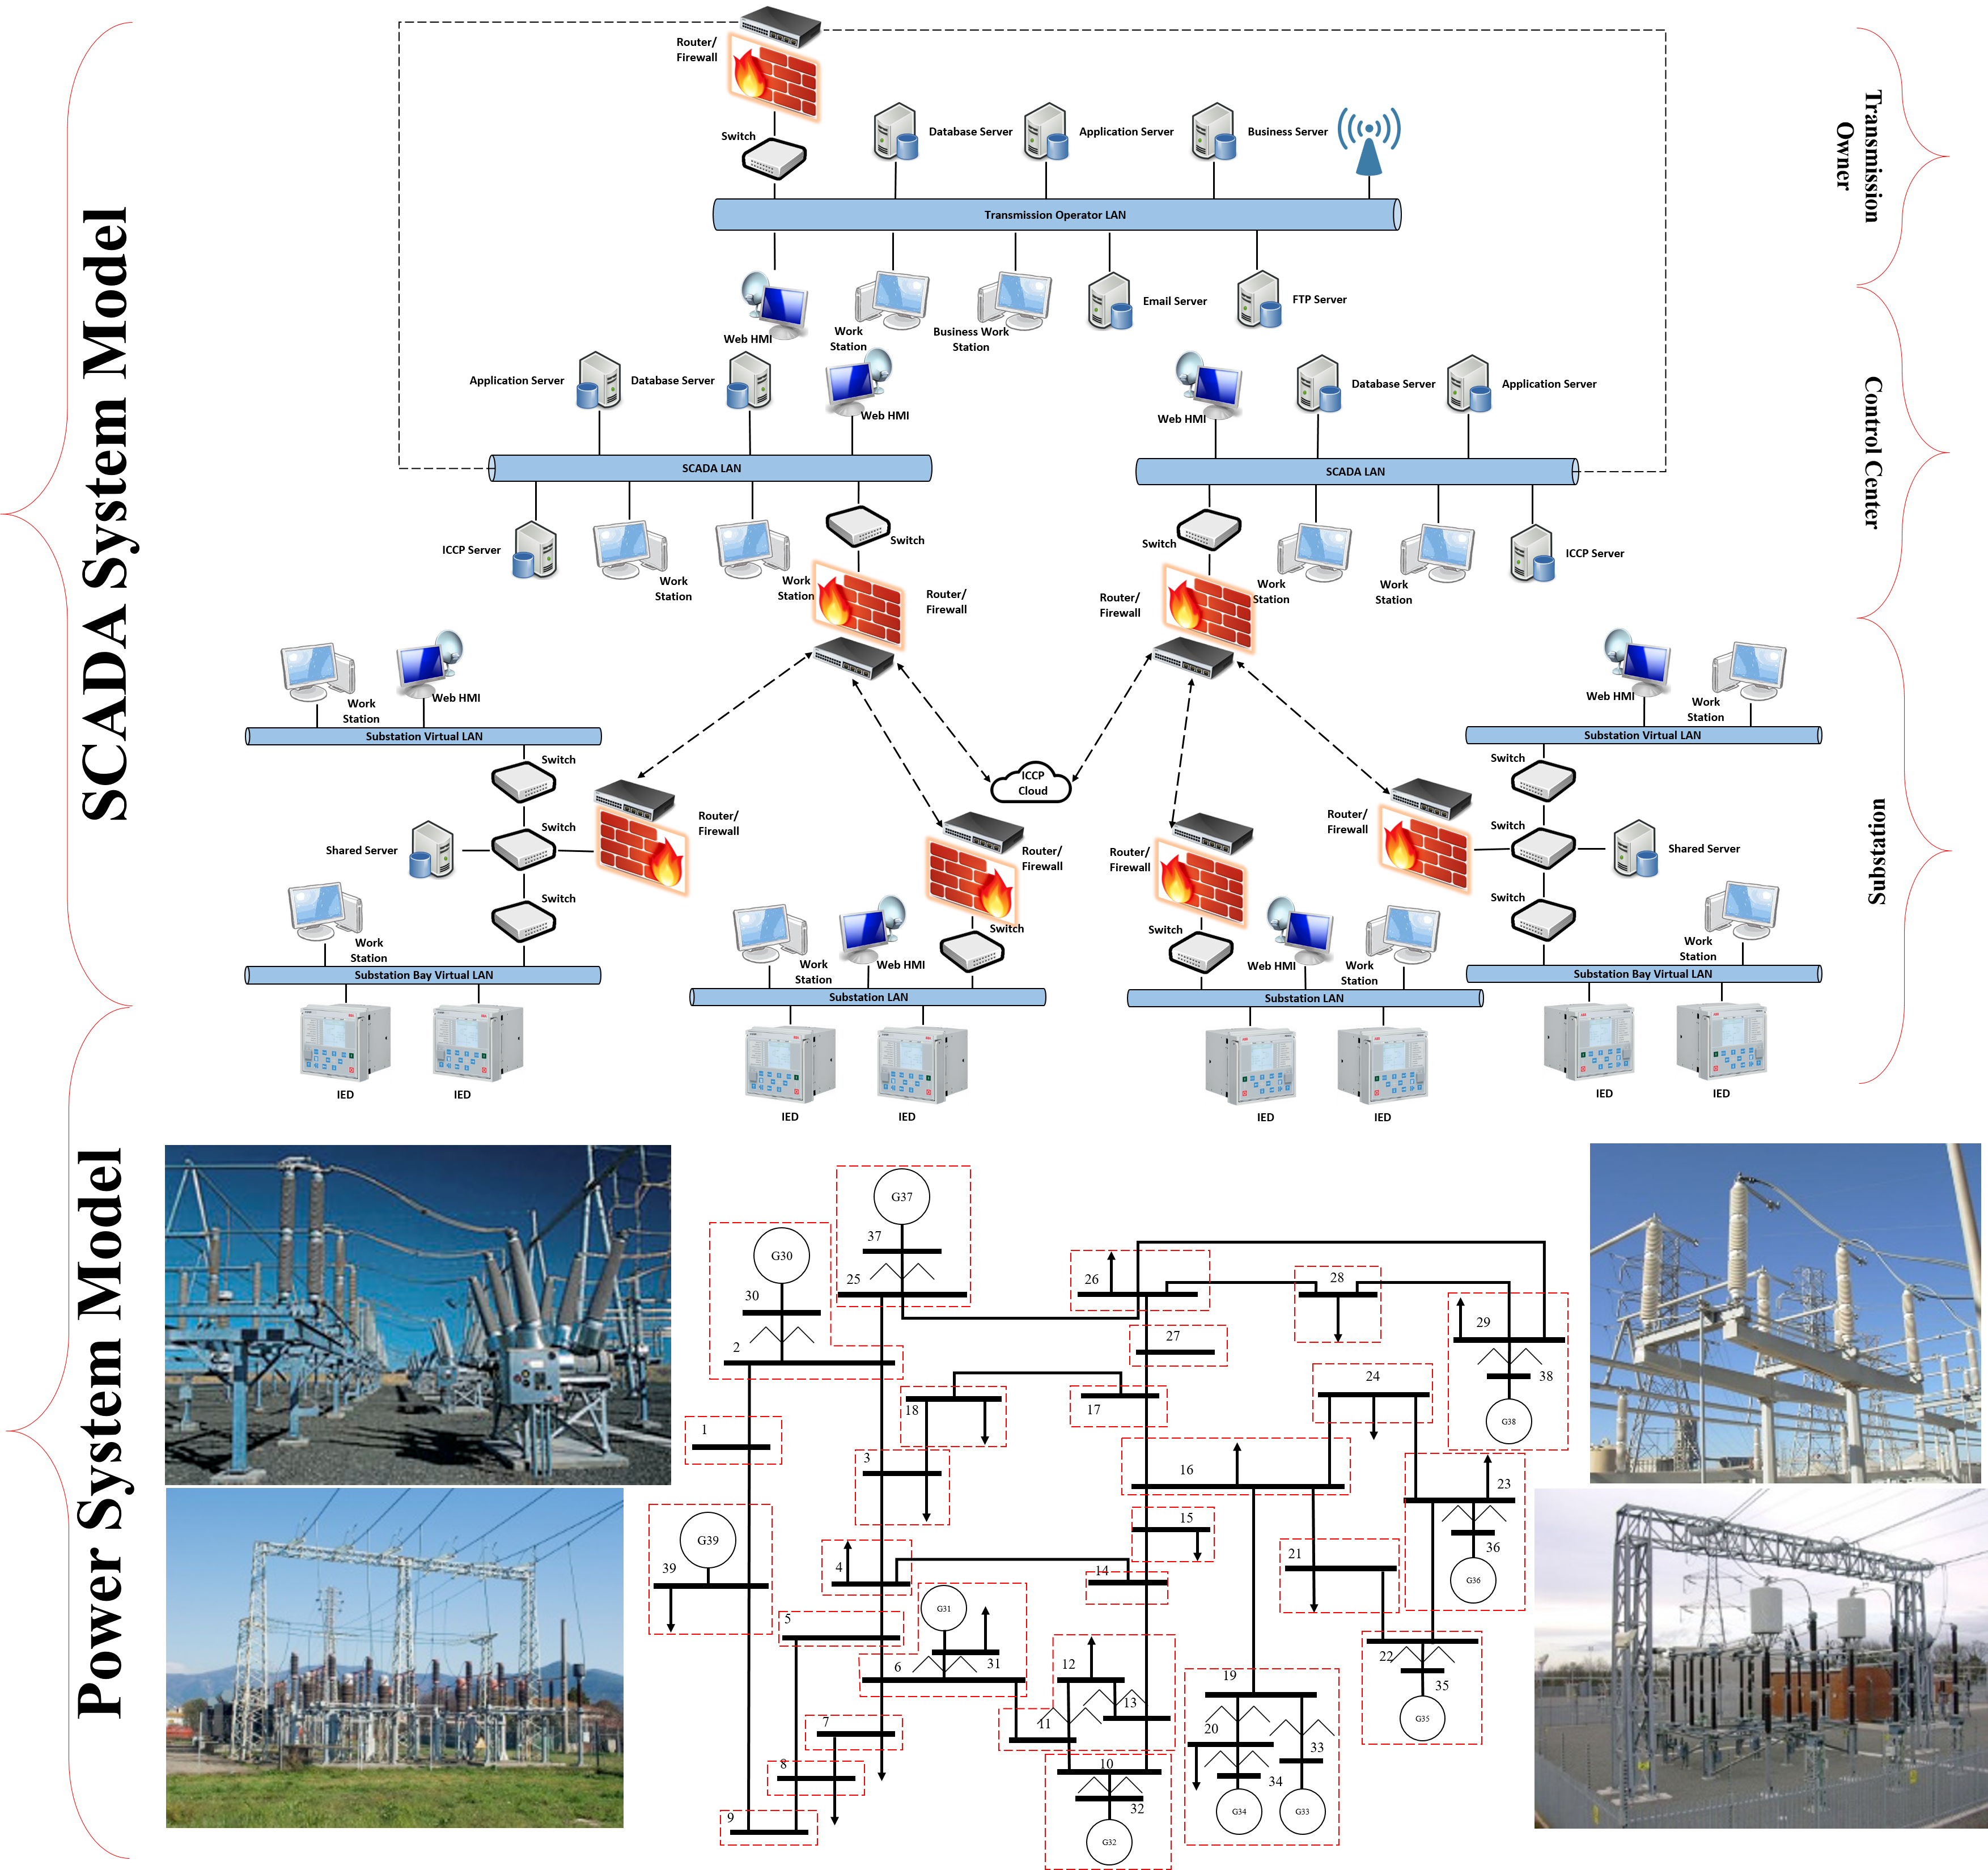
\includegraphics[width=0.42\textwidth]{fig-cyber-physical.png}
	\caption{Cyber-physical model of a typical power system.}
	\label{fig:cyber-physical}
\end{figure}

Several models have been proposed for identifying vulnerabilities in the CPS by evaluating the impact resulted from a cyber attack~\cite{stanley_2018,maninmiddle,petrinet1,petrinet2,Sridhar2012,alex1,alex2,alex3}. A very simple statistical model based on graph theory results has been proposed in~\cite{stanley_2018} where neither the SCADA nor the power network is accurately modeled. A Petri Net based cyber model consisting of firewalls and passwords has been proposed in~\cite{petrinet1}. Though the model was capable of replicating the operation of firewalls precisely, the probability of intrusion through a firewall was randomly selected irrespective of the hierarchy at which it is present. An improved usage of hierarchical Petri Nets is seen in~\cite{petrinet2} where the vulnerabilities of smart meters are modeled. However, the model was not developed to be applicable in the hierarchy of the SCADA system for the power grid. A comprehensive CPS model has been used in \cite{alex1,alex2,alex3} where every element of the communication system is modeled using queues. The attack efficiency of a possible cyber threat is evaluated as the time required to send a packet of data from the source vulnerability to the target. However, the time of arrival of the data packet is selected randomly based on the processing rate. Therefore, the relative difficulty in exploiting a particular vulnerability is not considered; nor the skill level of the intruder is used to determine the time to compromise a target vulnerability. To this end, a statistical model is proposed in~\cite{mcqueen} where the skill level of the intruder and the difficulty of exploiting a vulnerability is considered to determine the time to compromise a given vulnerability.

\textbf{Contribution.}\ In this work, a Bayesian attack tree based CPS model would be considered. The important vulnerabilities in the SCADA network would be first identified and then the attack path to a target goal would be evaluated. The probability of successfully exploiting a vulnerability would be calculated based on its type (relative difficulty to exploit) and the time to compromise it would be evaluated depending on the skill level of the intruder. The risk of the cyber vulnerabilities would be measured as the combined impact on both the cyber system and the power grid. Such a model would avoid comprehensive modeling of every element in the cyber system and would emphasize the modeling of the possible attack paths through the critical vulnerabilities.

The remainder of the proposal is organized as follows. Section~\ref{sec:prelim} discusses about the necessary preliminaries for the technical approach outlined in the proposal. Section~\ref{sec:technical} discusses about the cyber system and the physical system models which has been used for performing the security analysis. Finally Section~\ref{sec:simulation} details the simulation results for the proposed methodology.